
\chapter{Background Theory}

\label{ch:background}

\section{Models of Perfect Periodic Crystal Structures}\label{perfect_periodic}
Refer to: pg 28 29 35 \cite{thin_film_Boer}\\

Theoretical models of crystalline solids are based around the existence of translational symmetry in a crystal lattice such that the lattice can be constructed by periodically repeating a unit cell of atoms. The Bravais lattice specifies the periodic array in which the repeated units of the crystal are arranged. A crystal lattice can therefore be described by its underlying Bravais lattice and the arrangement of atoms, ions or molecules within a particular unit cell, i.e. the basis \cite{AshcroftMermin2}. This principle is used in a number of ways during this study. Firstly, this process is performed on a finite scale to construct a 64 atom supercell of CZTS from the 8 atom primitive unit cell for use in density functional theory (DFT) calculations to predict defect formation energy. This process is discussed further in section \ref{supercell_section}. The principle is also used in all DFT calculations of solid state systems through the implementation of periodic boundary conditions to simulate an infinite, bulk system using only a finite unit cell.\\
 
Another important concept in the theoretical modelling of periodic structures is reciprocal space and the reciprocal lattice. 
Converting to reciprocal space enables the description of periodic features with a longer-range periodicity than the unit cell in real space, such as the motion of electrons in a crystal and phonons.
In the same way that any quantity that varies with time can be described as a sum of Fourier components in the frequency domain; the spatial properties of a crystal can be described as a sum of components in Fourier space, otherwise known as reciprocal space or \textit{k}-space. The reciprocal lattice of a perfect single crystal is an infinite periodic 3D array of points whose spacings are inversely proportional to the distances between the planes in the lattice in real space. Vectors in real space have dimensions of length, whereas vectors in reciprocal space have dimensions of length$^{-1}$. This can therefore be compared directly to the wavevector $ \left(k  = \frac{2\pi}{\lambda} \right)$ of an excitation such as a phonon or a moving electron and multiplication of each coordinate of the reciprocal lattice by $\hbar$ converts reciprocal space into momentum space as for a quantised wave $\mathbf{p} = \hbar \mathbf{k}$ \cite{Blakemore1}. \\ 

\begin{figure}[h!]
  \centering
    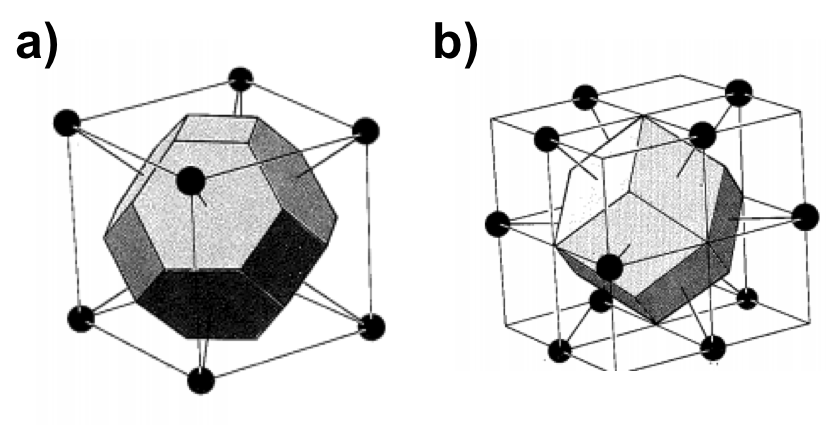
\includegraphics[width=0.5\textwidth]{figures/Wigner-Seitz.png}
    \caption{The Wigner-Seitz cell for the body-centred cubic Bravais lattice where there is a lattice point at its centre and on each vertex. The hexagonal faces bisect the lines joining the central point to the points on the vertices. The square faces bisect the lines joining the central point to the central points in each of the six neighbouring cubic cells. Figure taken from reference \citenum{AshcroftMermin2}.}
  \label{Wigner-Seitz}
\end{figure}

The Wigner-Seitz primitive cell is the most common choice of primitive cell with the full symmetry of the Bravais lattice. It represents the region of space around a lattice point  that is closer to that point than to any other lattice point. For example, figure \ref{Wigner-Seitz}a shows the truncated octahedron that is the Wigner-Seitz cell for a body-centred cubic (bcc) lattice \cite{AshcroftMermin2}.
The first Brillouin zone is the Wigner-Seitz primitive cell of the reciprocal lattice. The reciprocal of the bcc lattice is face-centred cubic (fcc), therefore the first Brillouin zone of  of the bcc lattice is the fcc Wigner-Seitz primitive cell as shown in figure \ref{Wigner-Seitz}b \cite{AshcroftMermin3}. As the full symmetry of the reciprocal lattice is contained within the first Brillouin zone, it is only necessary to sample \textit{k}-points within this single unit cell of the reciprocal lattice when calculating the electronic ground state of a periodic structure.

 
\section{Band Theory \& Band Structure of Semiconductors}\label{band_theory}
Refer to: pg 18 \cite{fund_semi}, pg 105 112 128 131 137 \cite{thin_film_Boer}, pg 111 + 119 \cite{phys_semicond}\\

The band theory of solids provides a means to explain the difference in the electrical conductivity of conductors, semiconductors and insulators. Electrons bound to an atom have a number of possible discrete energy levels. When a large number of atoms are brought together to form a solid, it becomes impossible to assign individual electrons to individual atoms. Instead, the electrons are considered to be shared amongst the atomic nuclei. However, a consequence of this sharing would be a large number of electrons occupying the same energy state, which violates the Pauli Exclusion Principle. The original discrete energy levels therefore are broadened into bands. The new energy levels are so closely spaced that they are considered to be a quasi-continuous band of allowed energies. This is illustrated in figure \ref{band_Elevels}. The series of bands of allowed energies in a semiconductor or insulator are separated by bands of forbidden energy, known as the band gap, E$_g$, of the material \cite{dielectric1}. In the simplest model, the upper energy band (the conduction band) is separated from the lower energy band (the valence band) by a constant band gap. This is called the flat band model. In real structures, the band architecture is more complicated than this simple model \cite{Tilley}.\\

\begin{figure}[h!]
  \centering
    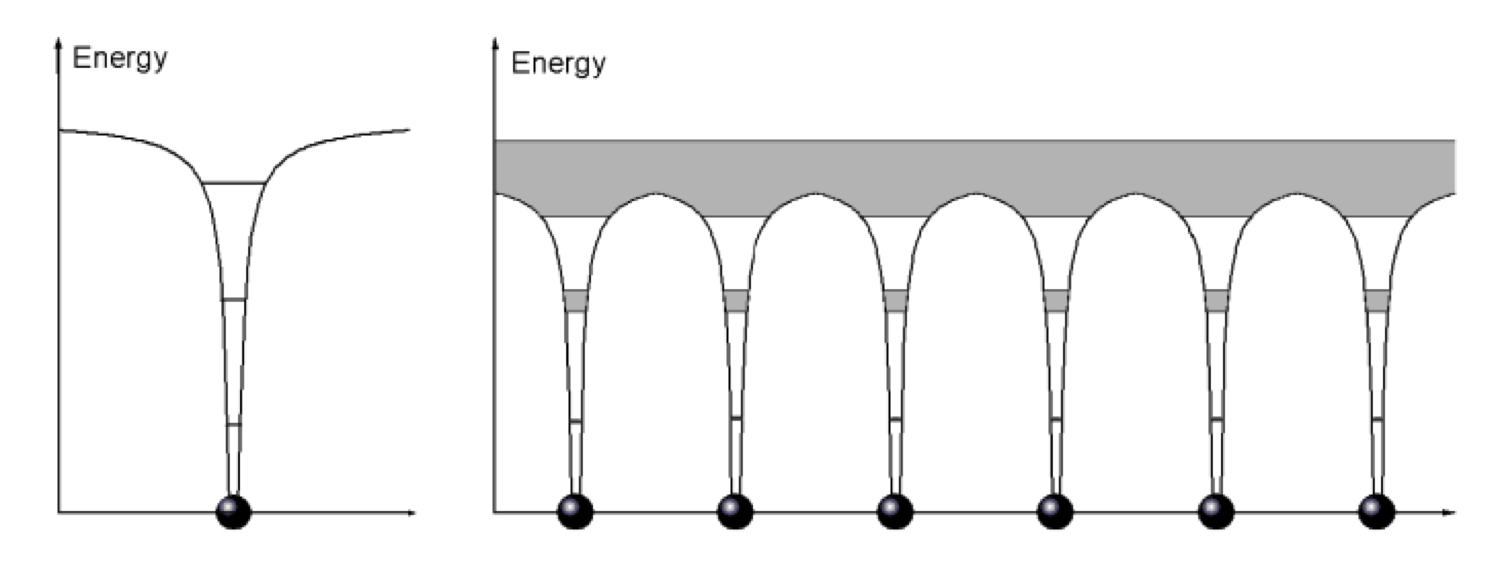
\includegraphics[width=0.7\textwidth]{figures/band_Elevels.png}
    \caption{Electron energy levels of a single atom (left) and the formation of a quasi-continuous band of allowed energies in a solid crystal when many atoms are brough close together (right). Figure taken from \citenum{mat_prop1}.}
  \label{band_Elevels}
\end{figure}

The concept of the energy band model of a solid emerges from considering the behaviour of electrons in a periodic crystal lattice, but cannot be understood in terms of classical physics alone. Instead, the electron must be considered in terms of wave-mechanical terms as a wave propagating in a periodic structure with diffraction and interference effects  \cite{small_semiconductor1}.
In the band theory of 
solids, the energy of a single electron in a perfect crystal is described by the one-electron Schr{\"o}dinger equation, shown in equation \ref{single_SE}. The first term in equation \ref{single_SE} is the kinetic 
energy of the electron, V(\textbf{r}) is the effective non-zero periodic potential energy experienced by 
the electron in the crystal, $\psi$ is the electron wavefunction and  $\epsilon$ is the eigenenergy of the electron. In band theory, it is assumed that for any electron, everything else in the crystal can be represented by the effective potential energy, V(\textbf{r}) \cite{Blakemore2}.
\begin{equation} \label{single_SE}
\left[ \left(-\frac{\hbar^2}{2m}\right)\nabla^2 + V(\mathbf{r})\right]\psi = \epsilon \psi 
\end{equation}
The spatial dependence of the potential experienced by an outer electron in a crystal for multi-electron systems was considered by Felix Bloch. He determined that the total potential is the sum of two parts. Firstly, the electrostatic potential due to the array of atomic cores. For a perfect lattice this should have the translational periodicity of the lattice. Secondly, the potential due to all other electrons. Bloch assumed that the charge density would have the same long-term average value in every unit cell of the crystal and therefore would be periodic. Bloch's theorem states that the wavefunction which satisfies equation \ref{single_SE} subject to a periodic potential should be of the form shown in equation \ref{bloch}, where $U_k(\mathbf{r})$ is some function 
(depending on the value of the wavevector, \textbf{k}) that also has the complete 
periodicity of the lattice and \textbf{k} is confined to the first Brillouin zone \cite{Blakemore2}.
\begin{equation} \label{bloch}
\phi_k(\mathbf{r}) = U_k(\mathbf{r}) e^{i\mathbf{k \cdot r}} 
\end{equation}
\begin{equation} \label{bloch_sum}
\psi_k(\mathbf{r}) = \sum_k A_k \phi_k(\mathbf{r}) = \sum_k A_kU_k(\mathbf{r}) e^{i\mathbf{k \cdot r}} 
\end{equation}
Due to the translational symmetry of a crystal lattice, an eigenfunction of the one-electron Schr{\"o}dinger equation can be expressed as a sum of Bloch functions such as that shown in equation \ref{bloch}, as shown in equation \ref{bloch_sum}. The one-electron wavefunctions therefore can be indexed by constants \textbf{k}, which are the wave vectors of the plane waves forming the `backbone' of the Bloch function. A plot of the electron eigenenergies from equation \ref{single_SE} versus \textbf{k} is known as the electronic band structure of the crystal \cite{fund_semi}.\\

\begin{figure}[h!]
  \centering
    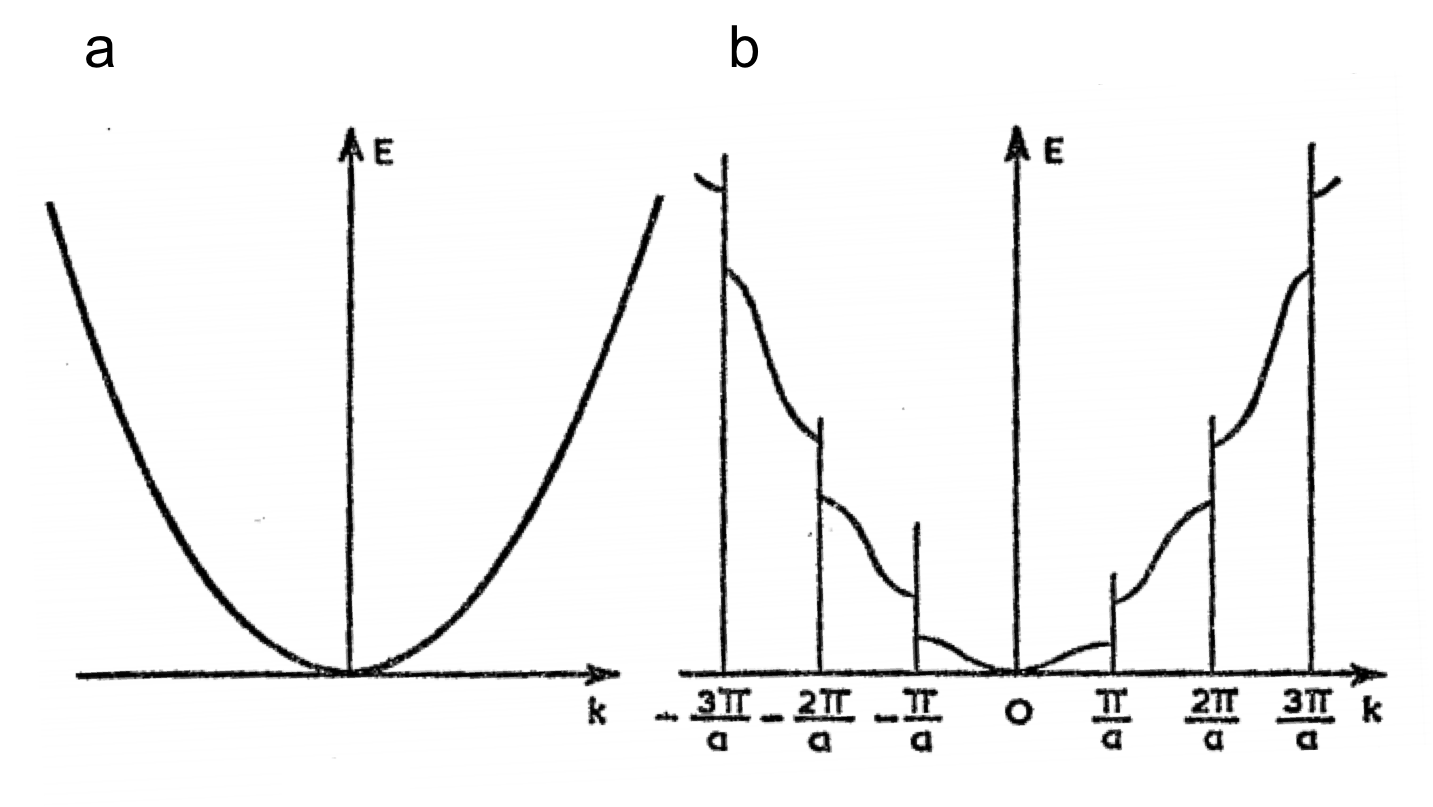
\includegraphics[width=0.7\textwidth]{figures/bs1.png}
    \caption{Energy-wave vector diagrams: (a) the free electron parabola, (b) modification due to a periodic crystal lattice. Figure taken from reference \citenum{small_semiconductor1}.}
  \label{bs1}
\end{figure}

The introduction of a medium with a discrete structure, such as a crystal lattice, has a profound effect on the dispersion relation of the waves. The energy dispersion relation of a free electron and that in a periodic crystal lattice is shown in figure \ref{bs1}. A periodic medium does not completely suppress the propagation of waves, as would be expected  in disordered or amorphous structures, but they do however introduce limiting frequencies and wavelengths for the propagation, followed by cut-off regions. The lower limit of the wavelength is set by the lattice spacing, a, giving an upper limit of the wave vector, \textbf{k}, of $\frac{\pi}{a}$. As figure \ref{bs1} shows, the parabola of the free electron in modified in a periodic crystal by the introduction of discontinuities at values of \textbf{k} corresponding to multiples of $\frac{\pi}{a}$. The appearance of such energy gaps implies that electrons in a periodic crystal may only have kinetic energies corresponding to certain bands, whilst being free to propagate in the lattice \cite{small_semiconductor2}.\\

Each electron occupies a state of definite $\mathbf{k}$. Therefore, an infinite number of electrons within the solid would result in an infinite number of \textit{k}-points. At each \textit{k}-point, only a finite number of the available energy levels will be occupied. Therefore only a finite number of electrons need to be considered but at an infinite number of \textit{k}-points. In practise, all of these \textit{k}-points are not considered. 
Electron wavefunctions will be almost identical for values of $\mathbf{k}$ that are sufficiently close, so the wavefunctions over a region of reciprocal space can be represented by considering the wavefunction at a single \textit{k}-point. It is therefore sufficient to consider the electronic states at a finite number of \textit{k}-points in order to determine the ground state energy of the solid. This approximation is illustrated in figure \ref{energy_dispersion}. Using Bloch's Theorem therefore has enabled the ground state energy to be determined by considering only the number of electrons in the unit cell at a finite number of \textit{k}-points, which are chosen to sample the Brillouin zone appropriately. The choice here is a balance between more \textit{k}-points for a more accurate representation of the Brillouin zone and fewer \textit{k}-points to reduce the computational expense of the calculation \cite{bloch-thesis}.\\

\begin{figure}[h!]
  \centering
    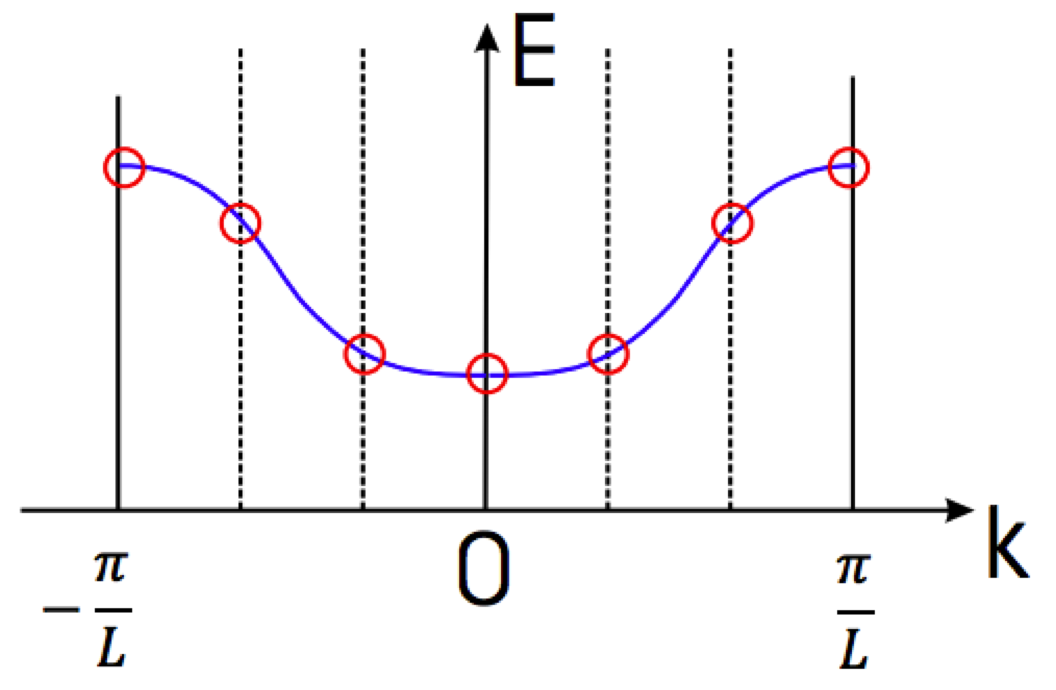
\includegraphics[width=0.4\textwidth]{figures/energy_dispersion.png}
    \caption{The energy dispersion relation for electrons moving in a crystal, illustrating how the function can be approximately represented by a finite number of \textit{k}-points, which form an equally-spaced mesh. Figure adapted from reference \citenum{vasp-slides}.}
  \label{energy_dispersion}
\end{figure}

A useful concept used to simplify the dynamics of an electron in a crystal lattice in the band theory of solids is that of effective mass, which was first mentioned in section \ref{PV_properties} as a key material property for a solar absorber material. The effective mass is a convenient parameter which accounts for the influence of a periodic lattice on a free carrier, enabling an electron in a periodic crystal to be treated as though it were a free particle but with a different mass in calculations of charge transport. Values of effective mass in semiconductors usually vary between 0.01 and 1 times the mass of a free electron and it is determined by the curvature of the energy graph in \textit{k}-vector space \cite{small_semiconductor2}. The effective mass is a parameter that can influence the efficiency of a solar cell, in particular, the effective mass of holes in the valence band and electrons in the conduction band (i.e. minority charge carriers) are of interest. The mobility of charge carriers is inversely proportional to the effective mass and the mobility of charge carriers in a PV material is important for efficient charge collection \cite{transport}.
 
 
 \section{Vibrational Properties of Semiconductors}
In section \ref{PV_properties}, effective mass and dielectric function were discussed for the insight these properties can provide for the likely PV performance of a material due to mobility of charge carriers in that material. However these are certainly not the only features of a real material at finite temperatures that need to be considered to understand carrier mobility in a material. At finite temperatures...lattice vibrations...called phonons. Electron-phonon interactions can heavily influence the optoelectronic properties of materials.
 
 'the interaction of charge carriers with lattice vibrations (phonons) is currently still a subject of intense debate16,17. Such electron–phonon interactions matter,
because they set a fundamental intrinsic limit to charge-carrier
mobilities in the absence of extrinsic scattering off impurities or interfaces18. `
 \cite{MAPI_Eg_broadening}
 
`charge-carriermobility m, which was found21–24
to scale with Tm with m in the range between ?1.4 and ?1.6. Several groups16,17,24 therefore proposed that electron–phonon coupling at room temperature is almost solely governed by deformation potential scattering with acoustic phonons, which is known18,25 to theoretically result in mpT?3/2.'
 \cite{MAPI_Eg_broadening}
 
 `In general, the two major mechanisms governing the electron–
phonon coupling in inorganic semiconductors are deformation potential scattering, in which distortions of the lattice change the electronic band structure'
 \cite{MAPI_Eg_broadening}
 As optical phonons in semiconductors typically have energies of the order of tens of meV (ref. 18), their population at low temperatures (To100 K) is very small; thus, homogeneous broadening in this regime predominantly results from acoustic phonons18,49
  \cite{MAPI_Eg_broadening}
  Long-wavelength acoustic phonons induce atomic displacements, which can correspond to macroscopic crystal deformation
   \cite{MAPI_Eg_broadening}


 
\section{Electronic Properties of Defects in Semiconductors}
Refer to: pg 160 \cite{fund_semi}, pg 51, 52, 64 \cite{thin_film_Boer}, pg 63 + 65 \cite{phys_semicond}\\

Although the main framework for materials modelling of solid-state systems (as was outlined in section \ref{perfect_periodic}) is built around perfect, periodic systems; in reality absolutely perfect systems do not exist. There is an energy cost associated with the creation of a defect, but in many cases the free energy of a system can be lowered by the incorporation of a certain concentration of defects due to an increase in the configurational entropy of the system \cite{AshcroftMermin_general}. 
At this point it is worth distinguishing between different types of defects for the purpose of later discussions.
Firstly, if a defect does not involve any atoms that are foreign to the host crystal, then the defect is called an intrinsic or native defect. Defects involving foreign atoms, or impurities, are referred to as extrinsic defects. In our study on {\CZTS} as we are first interested in the fundamental material properties we are currently only concerned with intrinsic impurities, although in real systems impurities are often unintentionally present in the growth or processing environment.
Defects are usually classified as point or line defects. Point defects usually involve isolated atoms in localized regions of a host crystal, whereas line defects involve rows of atoms, such as a dislocation defect. Another possible type of defect is a defect complex, which is composed of a small number of point defects. Some examples of defect complexes in {\CZTS} were shown in figure \ref{Chen_cluster1}. Defect complexes can be particularly interesting to study as there is some speculation in the literature that defects which are energetically less likely to form, could be more likely to form if they form a defect complex with defects that are more likely to form **find ref**.
There are then a number of different possible point defects, such as: vacancies, interstitials and antisites. In the case of our study on defects in {\CZTS}, it is sulfur vacancies ($V_{S}^{0}$, $V_{S}^{+}$, $V_{S}^{2+}$) and copper-on-zinc ($Cu_{Zn}^{-}$) and zinc-on-copper ($Zn_{Cu}^{+}$) antisites that are of interest, where  $Cu_{Zn}^{-}$ and $Zn_{Cu}^{+}$ form the charge neutral defect complex [$Cu_{Zn}^{-}$ + $Zn_{Cu}^{+}$]. The sulfur vacancy is an example of an electrically active defect. In this case the defect can contribute two free electrons to the host crystal and so is a donor or n-type defect.
**check** The free electrons can then either be fairly localized on the defect site to form a small polaron, or extended across several sites to form a large polaron, or be completely delocalized across the system **find ref**.\\

The electrical properties of semiconductors can be modified significantly by the incorporation of very small amounts of impurities or defects. It is often the case that less than one defect per million of host atoms is sufficient to alter the properties of a semiconductor \cite{fund_semi}. This sensitivity to defects is one of the reasons why semiconductors find many uses in device applications. For example, luminescence centres in wide-band-gap materials can be used to emit light at specific wavelengths or single-spin centres provided by defects can act as artificial atoms and serve as a qubit in a quantum information system \cite{defects_tutorial}. In order to control the electrical properties of a material by introducing defects, typically processes must first be developed to produce a fairly defect-free material, before introducing particular defects \cite{fund_semi}. However in the case of solar cell devices the presence of defects is typically detrimental. Various ways in which defects in the absorber material can impede solar cell performance are discussed further in section \ref{defects_in_PV} and more general characteristics of defects in semiconductors are discussed in the next section.

%\begin{itemize}
%\item Notes from A. Guinier 'X-Ray Diffraction' CH6 + Ziman
%\item Mention many types of disorder possible for multicomponent, especially for multi-component, compound semiconductor. e.g. of many types of possible defects for CdTe from Ken's work - and that's just binary!
%\item Extended defects usually detectable? 
%\item Discuss frozen in disorder and Scragg's work?
%\end{itemize}



\subsection{Impact of Defects on the Band Structure \& Optical Spectra}\label{PL_section}
 **See defect tutorial paper**\\


The energy band model, which was discussed in section \ref{band_theory}, has been successful in explaining many aspects of the behaviour of solids and a large amount of experimental data collected has supported the theoretical predictions made using the model. Its main drawback however is that is assumes a perfect, or nearly perfect, crystal lattice. It applies well to single crystals and polycrystalline substances, but cannot be applied to materials that are amorphous or heavily disordered so that the structure deviates significantly from the periodicity of the crystal \cite{small_semiconductor1}. Low concentrations of impurities and defects can be modelled by considering, for example, the introduction of additional donor and acceptor energy levels within the band gap of a material and the scattering of electrons and holes in the solid. However, at higher defect concentrations the band profile can be modified as shown in figure \ref{bs2} to give rise to conductivity even at temperatures that are too low to produce excitation of carriers into the free conduction bands, called impurity band conduction \cite{small_semiconductor2}.\\

\begin{figure}[h!]
  \centering
    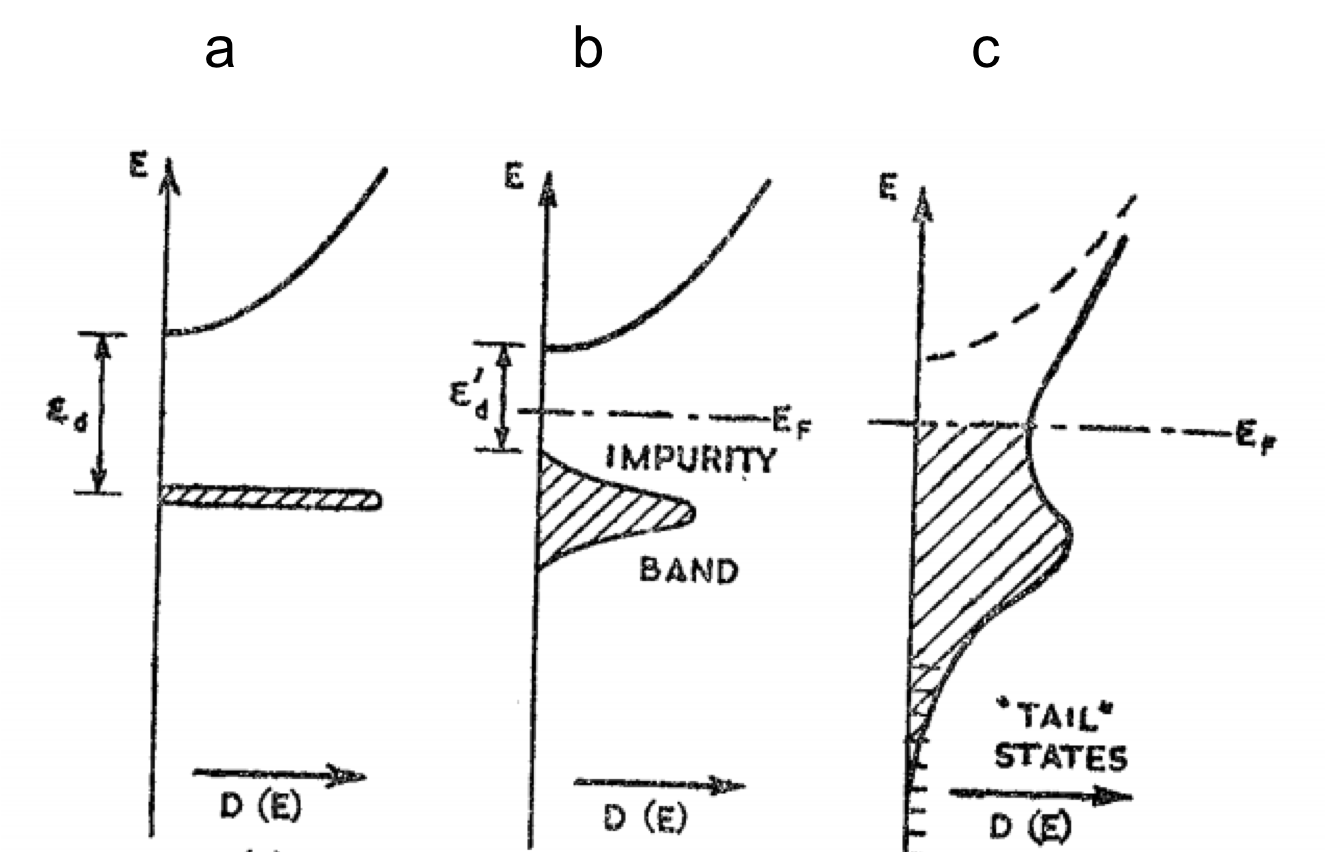
\includegraphics[width=0.7\textwidth]{figures/bs2.png}
    \caption{The influence of increased donor impurity density on the conduction band profile showing low (a), medium (b) and high (c) densities of impurities. Figure taken from reference \citenum{small_semiconductor2}.}
  \label{bs2}
\end{figure}

**Add in band tailing discussion from PL JC talk**\\





\subsection{Impact of Defects on Solar Cell Performance}\label{defects_in_PV}
Refer to: pg 217 221 \cite{thin_film_Boer}\\

Impact of Defects and Disorder on Photovoltaic Performance:
\begin{itemize}
\item Metal disorder in CZTS due to limited cooling/ annealing times, link to Jonathan Scragg's work (years to cool to perfect crystal)
\item SRH recomb, GBs, secondary phases, band gap and electrostatic potential fluctuations
\item See Culprit paper
\item See CMP lectures on defects + ebook reading material 
\end{itemize}

Band Tailing in Disordered Semiconductors:
\begin{itemize}
\item See culprit section 6.1 on Urbach tails
\item Nelson, pg 65, 3.5.4: heavy doping leading to band tailing
\item see Pankove + Russian 1970s papers, Urbach tail, fluctuations in electrostatic potential
\item See Urbach tail doc (pg 36) and use Cu/ Zn culprit paper + link to eris
\item See desktop papers from Jarv x2
\end{itemize}


\subsection{Photoluminescence Spectra of \CZTS}\label{CZTS_PL_section}
See word doc overview\\

Refer to: pg 10 \cite{spatial_resolved_book}, pg 345 \cite{fund_semi}\\

\begin{itemize}
\item See above books + old transfer report
\item Cardona, S7.1 Emission Spectroscopies
\item Photoluminescence (PL) imaging is becoming a popular method to inspect solar cell materials, it does not require a full functioning device and can be a powerful tool for probing defects in semiconductors \cite{characterization_book, Gerschon}. The PL spectra of \CZTS (CZTS) provides clear evidence of disorder in the material.
\item Overview of technique, information gained from technique, T dependent PL, PL spectra of CZTS: single crystal and thin film.
\end{itemize}

Photoluminescence (PL) spectroscopy is an example of a spatially resolved characterization technique, which can be used to give spatial information on the inhomogeneities in a PV device that cause a reduction in expected performance parameters, such as the $V_{OC}$.
PL is an imaging technique involving a one-step acquisition of the local properties of a whole PV device using an imaging device, compared to the typically lengthy step-by-step procedures required in scanning techniques, such as electron beam induced current (EBIC) and light beam induced current (LBIC). Luminescence imaging techniques involve using an imaging device to capture the photons emitted by radiative recombinations following the excitation of charge carriers in PV devices. In the case of PL, light is used for the excitation whereas in electroluminescence (EL) charge carriers are electrically excited. For an EL measurement therefore, the PV material must have electrical contacts. PL however is a contactless method and so firstly neglects the effects of the contacts on the conversion efficiency distribution but secondly can be carried out during earlier stages of the manufacturing, i.e. before the electrical contacts have been made \cite{spatial_resolved_book}.



PL is a particularly common characterisation technique used on CZTS with several such studies having been performed already. References \citenum{Gershon2, Gokmen, Halliday, PL, Romero} are just some examples of such studies. Low temperature PL specifically is a powerful tool for probing defects in semiconductors \cite{Gershon1} and ...\\
Notes from Pankove, notes from JC talk, figure showing common PL recombination mechanisms.

PL measurements have been performed on both polycrystalline CZTS \cite{Romero, Miyamoto, Unold} and single crystals of CZTS \cite{Halliday, Levcenko, Hones}. Polycrystalline samples are more similar to those likely to be used in thin-film CZTS photovoltaic devices, however comparison between those measurements with single crystal measurements could enable the isolation of recombination at grain boundaries from those due to bulk defects and secondary phases present within a single grain... relate to earlier section on polycrystalline thin-film PV\\

However, there is some disagreement in the literature about the main recombination mechanisms that could explain the observed PL spectra.

(mention two models of QDAP and elec pot fluc, Eg and charged defect induced + relate to Cu-Zn disorder)\\


%\subsection{Modulation Spectroscopy \& Band Gap Broadening}
%See pdf from Laurie - method used by PVTEAM to measure band gap broadening of CZTS single crystal + see quantum processes in semiconductors pg 244




%\section{Novel Optoelectronic Phenomena for High Performance Solar Cells}


%\subsection{Spin Orbit Interaction \& Rashba Splitting}\label{SOC_section}
%Refer to: pg 13 + 21-22 \cite{Bechstedt} + quantum processes in semiconductors pg 13 for SOC\\

% see webpages: pg 84 for discussion of effect of SOC on lattice without inversion symmetry!  + useful slide

%Look for textbook source?

%See rashba splitting paper (pre-Duke visit papers)

%\subsection{Photovoltaic-Ferroelectric Phenomena}\label{FE_PV_section}

%Ferroelectric PV materials are currently receiving a great deal of research interest, however the origin of their PV properties are considered to be unresolved \cite{Rappe}. A large number of theories have been proposed in an attempt to explain the two observed ferroelectric-photovoltaic (FE-PV) phenomena: the bulk PV effect (BPE), also referred to as the photogalvanic effect, and the anomalous PV effect (APE). In the BPE, a direct current appears in a homogeneous medium under uniform illumination and this can occur in all materials without a center of symmetry  \cite{PGE}. Ferroelectric materials exhibit this effect strongly \cite{Rappe} and the first observation of this effect was in 1956 with photovoltages measured in un-doped single crystals of the ferroelectric material BaTiO$_3$ \cite{keith_46}. In the case of the APE, photovoltages have been measured that are orders of magnitude larger than the band gap of the material \cite{keith_54}, but has been observed to disappear when the sample undergoes a phase transition to a paraelectric phase \cite{nonlinear_dielectric}, and so no longer exhibits spontaneous electric polarization. Theories have been developed to explain the FE-PV phenomena based around experimental observations of factors that have been shown to influence the photovoltage of FE-PV devices, such as:  the distance between the two opposite electrodes \cite{rev_28,rev_46}, intensity of incident light \cite{rev_47}, electrical conductivity \cite{Fridkin}, remnant polarization of the
%ferroelectric crystals \cite{rev_48}, crystallographic orientation \cite{rev_49}, the dimension or size of the crystals \cite{rev_46, rev_50}, domain walls \cite{rev_30} and the interface between the FE material and the electrode \cite{rev_37}.\\

%Models have been proposed to explain the BPE in ferroelectric materials based upon the built-in asymmetry of non-centrosymmetric crystals. One model is based on asymmetric scattering centres in the materials \cite{PGE}. In non-centrosymmetric crystals, the rate of the generation of charge carriers with momenta $\pm$k can be different due to asymmetric electron-hole scattering. A `ballistic current' can then be generated due to the momentum imbalance \cite{shift_current}.
%Another model, the shift current model \cite{shift_current}, has been proposed, which is based on the asymmetry of the electron density \cite{keith}.
%Light-induced transitions of charge carriers between bands in reciprocal space are accompanied by asymmetrical shifts in real space between atoms in elementary cells \cite{shift_current}.
%Such currents have been demonstrated for a number of materials, such as GaAs \cite{keith_52} and BiFeO$_3$, where this has been demonstrated using both computational \cite{keith_25} and experimental \cite{keith_51} techniques. \\

%The domain wall theory has been proposed to explain the large generated photovoltages in the APE \cite{domain_wall} and the Schottky-junction effect \cite{schottky_effect} and depolarization field model \cite{screen_effect, depol_model}, also referred to as the screening effect, have been proposed as additional contributions to the large photovoltage. Unlike the BPE, some theories to explain the APE rely on the nano- and microstructure of the material \cite{keith}. The latter two theories are related to the interface between the FE material and an electrode in a FE-PV device, but were originally neglected as the contributions to the photovoltage were believed to be small. However, these effects become more significant in thin-film devices where photovoltages are typically low \cite{FE_PV_rev1}, and thin-films are particularly relevant for PV applications.\\

%The domain wall theory was developed to explain observations of photovoltages in thin films of BiFeO$_3$ increasing linearly with the total number of ferroelectric domain walls along the net direction of electric polarization and vanishing along the direction perpendicular to the net polarization \cite{rev_30}. In this theory, the narrow ferroelectric domain walls drive the dissociation of photogenerated excitons and so  act as nanoscale photovoltage generators connected in series. The photocurrent across the domain walls is therefore continuous but the photogenerated voltage accumulates along the direction of net polarization, allowing for photovoltages that are considerably larger than the band gap of the material \cite{FE_PV_rev1}.
%In the Schottky-junction effect, the FE semiconductor forms a Schottky contact with the metal electrodes, which then generate a photocurrent under illumination due to the local electric field caused by the band bending near to the electrode. This photocurrent is dependent upon the Schottky barrier height and depletion region depth, but the photovoltage is still limited to the band gap of the material. Further, the additional photovoltage contribution from this effect can be cancelled out if the same electrode contacts are used, due to the opposite polarization of the two Schottky-junctions \cite{FE_PV_rev1}.
%In the depolarization field model, high densities of polarization charges are believed to accumulate on surfaces of polarized FE films, this then induces a large electric field inside the FE layer if the charge is not screened. This effect will be far more pronounced in a thin-film device. The electric field is thought to not be fully screened by the free charges in the metal or semiconductor that the FE layer is in contact with, resulting in a depolarization field. This depolarization field will be larger when the FE material has a large remnant electric polarization, the FE layer is thinner and when it is in contact with a semiconductor, as opposed to a metal, due to fewer free charge carriers and higher dielectric constant in a semiconductor than a metal, giving weaker screening. The depolarization field is believed to be the dominating force for the separation of photogenerated charge carrier pairs \cite{FE_PV_rev1}.\\

%Clearly the exact mechanism behind the observed PV phenomena in FE materials are not yet fully understood, but they could open up new possible routes for materials to enable higher performance solar cells. In particular, the APE could be utilized for materials with higher V$_{OC}$ to enable a higher power output from a solar cell. Additionally, it has been suggested that ferroelectric domains may be able to drive the separation of photoexcited electron-hole pairs to reduce detrimental recombination in solar absorber materials \cite{Jarv}. 